\documentclass[11pt]{article}
\usepackage{worksheet_style}

% ---- Toggle: uncomment for filled version ----
%\worksheetfilledtrue
\begin{document}
\worksheetheader{6}{Motion Along a Curve \& Arc Length}

\begin{background}
Last time we defined vector-valued functions and their derivatives. Today we put them to work: the derivative $\vect{r}'(t)$ gives velocity, its magnitude gives speed, and integrating the speed gives arc length. We also derive the projectile motion equations you may have seen in physics---but now with the full vector calculus treatment.
\end{background}

%=============================================================
\wsection{Kinematics of Space Curves}

\begin{defbox}{Position, Velocity, Acceleration}
For a particle moving along $\vect{r}(t)$:

\begin{tabular}{lll}
  \textbf{Position:} & $\vect{r}(t)$ & where the particle is \\
  \textbf{Velocity:} & $\vect{v}(t) = \wbm{\vect{r}\,'(t)}$ & direction and rate of movement \\
  \textbf{Speed:} & $\|\vect{v}(t)\| = \wbm{\|\vect{r}\,'(t)\|}$ & how fast (scalar!) \\
  \textbf{Acceleration:} & $\vect{a}(t) = \wbm{\vect{v}\,'(t) = \vect{r}\,''(t)}$ & rate of change of velocity
\end{tabular}
\end{defbox}


\begin{formulabox}{Recovering Position from Velocity/Acceleration}
\[\vect{v}(t) = \int \vect{a}(t)\,dt + \vect{C}_1 \qquad \vect{r}(t) = \int \vect{v}(t)\,dt + \vect{C}_2\]
-- Use initial conditions $\vect{v}(0)$ and $\vect{r}(0)$ to find the constants
\end{formulabox}

-- \textbf{Displacement} (net change): $\ds\int_a^b \vect{v}(t)\,dt$ -- a vector

-- \textbf{Total distance traveled}: $\ds\int_a^b \|\vect{v}(t)\|\,dt$ -- a scalar (always $\geq$ displacement magnitude)

\begin{example}[Displacement vs.\ Distance]
A particle has velocity $\vect{v}(t) = \vec{3t, 4, t^2}$ on $[0,2]$.
\begin{enumerate}[label=(\alph*), nosep]
  \item Find the displacement.
  \item Set up the integral for total distance traveled.
\end{enumerate}

\wbbox{
\textbf{(a) Displacement:}

1. Integrate each component:
\[\int_0^2 \vect{v}(t)\,dt = \left\langle\left[\frac{3t^2}{2}\right]_0^2, [4t]_0^2, \left[\frac{t^3}{3}\right]_0^2\right\rangle = \vec{6, 8, \frac{8}{3}}\]

\textbf{(b) Total distance:}

1. Speed: $\|\vect{v}(t)\| = \sqrt{9t^2 + 16 + t^4}$

2. Integral: $\ds\int_0^2 \sqrt{9t^2 + 16 + t^4}\,dt$ -- no nice closed form, use numerical methods.
}{5cm}
\end{example}

%=============================================================
\wsection{Arc Length}

\begin{thmbox}{Arc Length of a Parametric Curve}
\textbf{Idea.} Approximate the curve by a chain of tiny straight segments. Each segment between $\vect{r}(t)$ and $\vect{r}(t+dt)$ has length $\|\vect{r}\,'(t)\|\,dt$ (velocity times time). Adding these up in the limit gives the total arc length:
\[L = \int_a^b \|\vect{r}\,'(t)\|\,dt = \wbml{\displaystyle\int_a^b \sqrt{\left(\frac{dx}{dt}\right)^2 + \left(\frac{dy}{dt}\right)^2 + \left(\frac{dz}{dt}\right)^2}\,dt}\]
\end{thmbox}

\begin{center}
\begin{tikzpicture}[scale=1.0]
    \draw[thick, domain=0:8, smooth, variable=\x, blue] plot ({\x}, {sin(deg(\x/4)) + 2});
    \coordinate (A) at (2, {sin(deg(2/4)) + 2});
    \coordinate (B) at (4, {sin(deg(4/4)) + 2});
    \coordinate (B_proj) at (4, {sin(deg(2/4)) + 2});
    \draw[red, thick] (A) -- (B) -- (B_proj) -- cycle;
    \draw[-] (A) -- (B) node[midway, above] {$\Delta s$};
    \draw[-] (B_proj) -- (B) node[midway, right] {$\Delta y$};
    \draw[-] (A) -- (B_proj) node[midway, below] {$\Delta x$};
    \draw[->] (-0.5,0) -- (9,0) node[right] {$x$};
    \draw[->] (0,-0.5) -- (0,4) node[above] {$y$};
    \filldraw[black] (A) circle (1pt) node[below left] {$(x, y)$};
    \filldraw[black] (B) circle (1pt) node[above right] {$(x+\Delta x, y+\Delta y)$};
    \draw[dashed] (B) -- (B_proj);
\end{tikzpicture}\\
{\small Approximating the arc length of a curve using a right triangle with $\Delta s$ as the hypotenuse, $\Delta x$ as the base, and $\Delta y$ as the height. Summing $\Delta s$ over infinitely many such triangles gives the integral formula for $L$.}
\end{center}

\begin{formulabox}{Arc Length in Other Coordinates}
\textbf{Cartesian} ($y = f(x)$):
\[L = \wbml{\displaystyle\int_a^b \sqrt{1 + \left(\frac{dy}{dx}\right)^2}\,dx}\]

\textbf{Polar} ($r = f(\theta)$):
\[L = \wbml{\displaystyle\int_\alpha^\beta \sqrt{r^2 + \left(\frac{dr}{d\theta}\right)^2}\,d\theta}\]
\end{formulabox}

\begin{example}[Arc Length of a Helix]
Find the arc length of $\vect{r}(t) = \vec{2\cos t,\; 2\sin t,\; 3t}$ for $t\in[0, 2\pi]$.

\wbbox{
1. Derivative: $\vect{r}\,'(t) = \vec{-2\sin t,\; 2\cos t,\; 3}$

2. Speed: $\|\vect{r}\,'(t)\| = \sqrt{4\sin^2 t + 4\cos^2 t + 9} = \sqrt{4+9} = \sqrt{13}$

3. Arc length: $L = \ds\int_0^{2\pi}\sqrt{13}\,dt = \boxed{2\pi\sqrt{13}}$

Note: the speed is constant -- the helix is traversed at a uniform rate.
}{4cm}
\end{example}

\begin{example}[Arc Length of a $t^2/t^3$ Curve]
Find the arc length of $\vect{r}(t) = \vec{t^2, t^3}$ for $t\in[0, 1]$.

\wbbox{
1. Derivative: $\vect{r}\,'(t) = \vec{2t, 3t^2}$

2. Speed: $\|\vect{r}\,'(t)\| = \sqrt{4t^2+9t^4} = t\sqrt{4+9t^2}$

3. Arc length:
\[L = \int_0^1 t\sqrt{4+9t^2}\,dt\]

4. Substitution: $u = 4+9t^2$, $du = 18t\,dt$:
\[L = \frac{1}{18}\int_4^{13} \sqrt{u}\,du = \frac{1}{18}\cdot\frac{2}{3}\left[u^{3/2}\right]_4^{13} = \frac{1}{27}\left(13\sqrt{13} - 8\right) = \boxed{\frac{13\sqrt{13}-8}{27}}\]
}{5cm}
\end{example}

%=============================================================
\wsection{Projectile Motion}

-- Projectile launched from origin, initial speed $v_0$, angle $\theta$ above horizontal, no air resistance

\begin{formulabox}{Projectile Motion Equations}
\begin{align*}
  \vect{r}(t) &= \wbml{\vec{v_0 \cos\theta\cdot t,\; v_0\sin\theta\cdot t - \tfrac{1}{2}gt^2}} \\[4pt]
  \text{Max height:} \quad H &= \wbml{\frac{v_0^2 \sin^2\theta}{2g}} \\[4pt]
  \text{Time of flight:} \quad T &= \wbml{\frac{2v_0\sin\theta}{g}} \\[4pt]
  \text{Range:} \quad R &= \wbml{\frac{v_0^2 \sin(2\theta)}{g}}
\end{align*}

-- Max range at $\theta = \wbm{45^\circ}$ \quad -- Max height at $\theta = \wbm{90^\circ}$
\end{formulabox}

\begin{center}
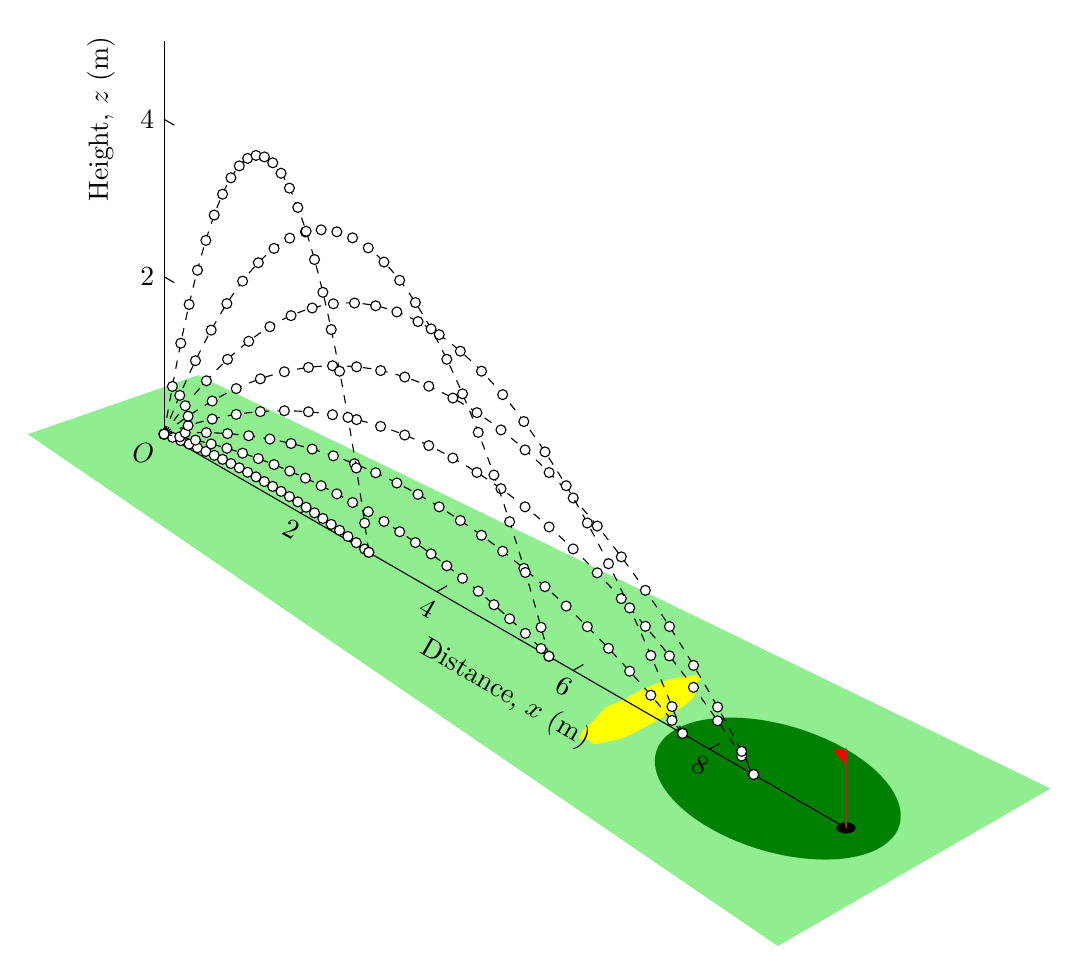
\begin{tikzpicture}[x=(330:1cm),y=(30:1cm),z=(90:1cm)]
    \fill [LightGreen] (-1,-1,0) -- (-.5,1,0) -- (11,2,0) -- (11,-2,0) -- cycle;
    \fill[Green] (9,0,0) circle [x radius=1.5, y radius=1];
    \fill[black] (10,0,0) circle [x radius=.1, y radius=.1];
    \draw[Brown, thick, line cap=round] (10,0,0) -- (10,0,1);
    \fill[Red] (10,0,1) -- (9.8,0,0.9) -- (10,0,0.8) -- cycle;
    \fill[Yellow, shift={(7,0,0)}]
        plot [domain=0:340, samples=20, smooth cycle, variable=\t]
            (\t:rnd/16+0.25 and rnd/8+0.75);
    \node[below left] {$O$};
    \draw (0, 0) -- (10, 0)
        node[midway, yshift=-.8cm, rotate=330] {Distance, $x$ (m)};
    \draw foreach \i in {2,4,6,8}
        { (\i, 0) node[below, rotate=330] {\i} -- ++(0, .15) };
    \draw (0, 0, 0) -- (0, 0, 5)
        node[pos=.8, xshift=-.8cm, rotate=90] {Height, $z$ (m)};
    \draw foreach \i in {2,4}
        { (0, 0, \i) node[left] {\i} -- ++(.15, 0, 0) };
    \foreach \a[evaluate={\v=70; \T=\v*sin(\a)/9.807*2;}] in {10, 20, ..., 80} {
        \draw[x=(330:0.5pt), z=(90:0.5pt), Black, dashed]
            plot [smooth, domain=0:\T, samples=50, variable=\t,
                  mark=*, mark repeat=2, mark size=1.8pt, mark options={fill=white, solid}]
                (\v*\t*cos \a, 0, -9.807/2*\t^2+\v*\t*sin \a +0.1016) coordinate (end);
        \filldraw[fill=White] (end) circle [radius=1.8pt];
    }
\end{tikzpicture}\\
{\small Projectile trajectories at several launch angles, shown on a golf course. In the absence of air resistance each ball follows a parabolic path; the $45^\circ$ launch gives the longest range.}
\end{center}

\begin{example}[Projectile Problem]
A ball is launched at $v_0 = 20$ m/s at $\theta = 45^\circ$. Find max height, time of flight, and range. ($g = 9.8$ m/s$^2$)

\wbbox{
1. Setup: $\sin 45^\circ = \cos 45^\circ = \frac{\sqrt{2}}{2}$

2. Max height: $H = \frac{20^2 \cdot (1/2)}{2(9.8)} = \frac{200}{19.6} \approx \boxed{10.2\text{ m}}$

3. Time of flight: $T = \frac{2(20)(\sqrt{2}/2)}{9.8} = \frac{20\sqrt{2}}{9.8} \approx \boxed{2.89\text{ s}}$

4. Range: $R = \frac{400\sin 90^\circ}{9.8} = \frac{400}{9.8} \approx \boxed{40.8\text{ m}}$

Note: $\theta=45^\circ$ maximizes range since $\sin(2\cdot 45^\circ) = 1$.
}{5cm}
\end{example}

%=============================================================
\vspace{6pt}
\textit{Show all work for full credit.}

\begin{practice}

\prob Find the velocity, speed, and acceleration of $\vect{r}(t) = \vec{\sqrt{t},\; t^3,\; e^t}$ at $t=1$.

\wans{$\vect{v}(1) = \wbml{\vec{1/2,\; 3,\; e}}$, \; speed $= \wbml{\sqrt{37/4+e^2}}$, \; $\vect{a}(1) = \wbml{\vec{-1/4,\; 6,\; e}}$}

\vspace{3cm}

\prob Find the arc length of $\vect{r}(t) = \vec{t,\; t^2/\sqrt{2},\; t^3/3}$ for $t\in[0,1]$.

\textit{Hint:} simplify $\|\vect{r}\,'(t)\|$ -- it factors.

\wans{$L = \wbm{4/3}$}

\vspace{3.5cm}

\prob Find the arc length of the cardioid $r = 1 + \cos\theta$ for $\theta\in[0,2\pi]$.

\textit{Hint:} use $1+\cos\theta = 2\cos^2(\theta/2)$.

\wans{$L = \wbm{8}$}

\vspace{3.5cm}

\prob A golfer hits a ball at $v_0 = 45$ m/s. What angle gives maximum range, and what is that range?

\wans{$\theta = \wbm{45^\circ}$, \; $R = \wbml{\frac{2025}{9.8} \approx 206.6 \text{ m}}$}

\vspace{2.5cm}

\prob A particle has $\vect{a}(t) = \vec{0, 0, -g}$, $\vect{v}(0) = \vec{3, 4, 10}$ m/s, $\vect{r}(0) = \vec{0, 0, 100}$ m. Find $\vect{r}(t)$ and the time it hits the ground ($z=0$).

\wans{$\vect{r}(t) = \wbml{\vec{3t,\; 4t,\; -\frac{g}{2}t^2+10t+100}}$}

Time: $t = \wbml{\frac{10+\sqrt{2060}}{9.8} \approx 5.65 \text{ s}}$

\vspace{3.5cm}

\end{practice}

\end{document}
